\chapter{Results}
\label{ch:results}

%% -----------------------------------------------------------------------------
%% -----------------------------------------------------------------------------
\section{Final Neural Network}
The 1,499 instances in the cleaned training data set and their corresponding attributes were used to develop an ANN with the optimized architecture given in \ref{table: archs 2}. The resulting network has twenty three input attributes, six neurons in the first hidden layer, two neurons in the second hidden layer and predicts the $ln(rate_{forward})$. The parity plots demonstrating the resulting fit of the optimized ANN are given in figures \ref{fig:Main NN with the training/testing data} for the training set and \ref{fig:Main ANN testing data} for the testing set.  
		\begin{figure}[!htbp]
		    \centering
		    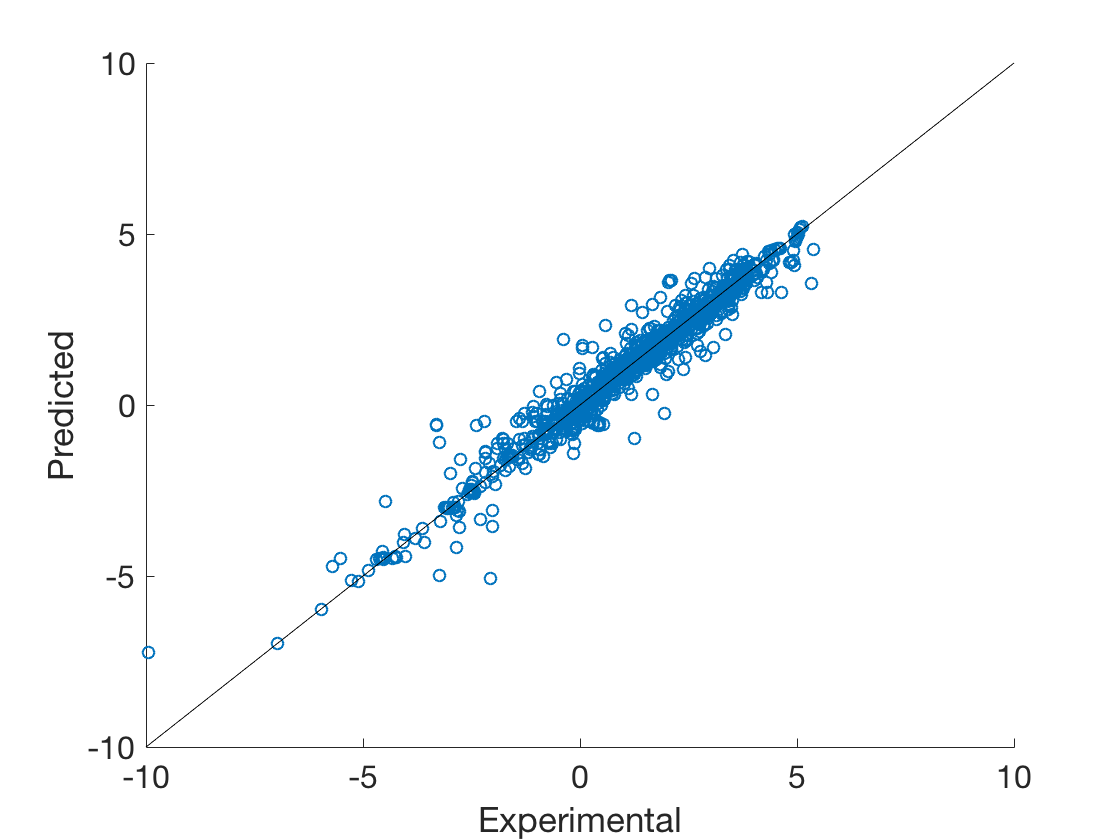
\includegraphics[width=0.7\textwidth]{Results/MainANN/Training_Results.png}
	        \caption{Parity plot for training performance of the ANN}
	        \label{fig:Main NN with the training/testing data}
			\end{figure}
		\begin{figure}[!h]
		    \centering
		    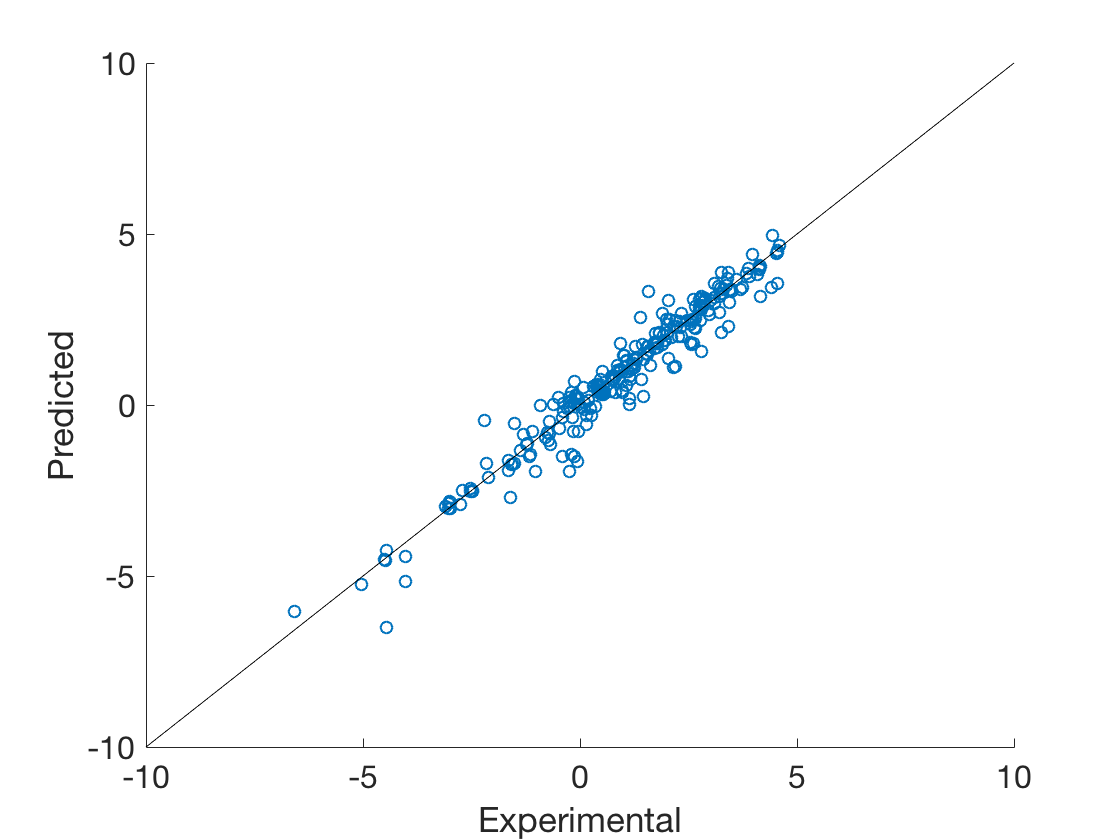
\includegraphics[width=0.7\textwidth]{Results/MainANN/Testing_Results.png}
	        \caption{Parity plot for testing performance of the ANN}
	        \label{fig:Main ANN testing data}
			\end{figure}
The corresponding errors are given in table \ref{table: training results}. Based on the error analysis, the model is not believed to be overtrained. This is consistent with the ratio of training data points to weights in the ANN. These results demonstrate that using the modified continuous attributes to describe each catalyst component, rather than categorically representing the data, results in comparable ANN performance.
		\begin{table}[!htbp]
			\centering
			\caption{Error Analysis from ANN Training}
			\label{table: training results}
			\begin{tabular}{c|cc}
			\textbf{Data Set} & \textbf{$R^2$} & \textbf{MSE} \\ \hline
			Training          & 0.945       & 0.232        \\
			Testing           & 0.946       & 0.240       
			\end{tabular}
			\end{table}
A sensitivity analysis was performed to evaluate the relative contribution of each attribute to the ANN. To determine this, each attribute was removed from the input data set. Then following the algorithm presented in the Methods section ($m=5$, $n=5$), the resulting ANN performance was evaluated. The results are given in table \ref{table: sensitivity analysis}. An increase in the MSE or decrease in the $R^2$ value from the base case indicates that the attribute contributes significantly to the ANN prediction. The attributes with the largest sensitivity were binding energy of carbon and reaction temperature. Removing the binding energy of carbon, which was used to relate the primary catalyst metals,led to an increase in the MSE from 0.42 to 0.58. The reaction temperature also contributed significantly to the predicted rate, increasing the MSE from 0.42 to 1.24. The MSE and $R^2$ reported for all other attributes are considered within reasonable error. 

\begin{table}[!htbp]
	\centering
	\caption{Sensitivity analysis results}
	\label{table: sensitivity analysis}
	\begin{tabular}{lcc}
	\textbf{Attribute}                 & \textbf{MSE} & \textbf{$R^2$} \\ \hline
	No Attributes Removed, Base Case   & 0.420        & 0.90                         \\ \hline
	Binding Energy Carbon              & 0.577        & 0.87                         \\
	Primary Metal Loading, wt\%        & 0.454        & 0.89                         \\
	Promoter Charge/Ionic Radius       & 0.385        & 0.91                         \\
	Promoter Electronegativity         & 0.366        & 0.92                         \\
	Promoter Loading, wt\%             & 0.348        & 0.91                         \\
	Support, First Ionization Energy   & 0.403        & 0.91                         \\
	Support, Electronegativity         & 0.414        & 0.90                         \\
	Synthesis                          & 0.419        & 0.90                         \\
	Calcination Temperature.           & 0.316        & 0.92                         \\
	Calcination Time                   & 0.415        & 0.90                         \\ \hline
	Reaction Temperature               & 1.244        & 0.70                         \\
	Reactant Feed, \ce{H2} vol\%            & 0.449        & 0.90                         \\
	Reactant Feed, \ce{CO} vol\%            & 0.430        & 0.90                         \\
	Reactant Feed, \ce{H2O} vol\%           & 0.446        & 0.90                         \\
	Reactant Feed, \ce{CO2} vol\%           & 0.371        & 0.91                         \\
	Time on Stream.                    & 0.357        & 0.92                         \\
	Total Inlet Flowrate/Catalyst Mass & 0.463        & 0.90                        
	\end{tabular}
\end{table}
\FloatBarrier
%% -----------------------------------------------------------------------------
%% -----------------------------------------------------------------------------
\section{Scaling Relations}
	\subsection{Following Scaling Relations}
	As with any scaling relation, the ANN can be used to predict the optimum catalyst that falls within the scaling relation. After training the model with the 1499 instances (neglecting \ce{Au/CeO2} and \ce{Pt/CeO2}),the optimum catalyst was determined by identifying the instance with the largest forward rate. The optimum catalyst was found to have the properties listed in table \ref{table: opt catalyst}. This corresponds to a 20wt\%Pt/\ce{Al2O3} catalyst promoted with 15wt\%Ni, synthesized using incipient wetness impregnation.

	\begin{table}[!htbp]
		\centering
		\caption{Optimum catalyst search results}
		\label{table: opt catalyst}
		\begin{tabular}{lc}
		\textbf{Attribute}                               & \textbf{Optimum} \\ \hline
		Binding Energy Carbon (eV)                       & -5.81            \\
		Primary Metal Loading (wt\%)                     & 0.2              \\
		Promoter Charge/Ionic Radius (charge/pm)         & 0.3571           \\
		Promoter Electronegativity (Pauling Scale)       & 1.91             \\
		Promoter Loading (wt\%)                          & 15               \\
		Support Metal, First Ionization Energy (kJ/mol)  & 577.50           \\
		Support Metal, Electronegativity (Pauling Scale) & 1.61             \\
		Synthesis Method                                 & IWI              \\
		Calcination Temperature (Celsius)                & 500              \\
		Calcination Time (hours)                         & 4                \\
		Reaction Temperature (Celsius)                   & 350              \\
		Reactant Feed, \ce{H2} vol\%                     & 0                \\
		Reactant Feed, \ce{CO} vol\%                     & 3                \\
		Reactant Feed, \ce{H2O} vol\%                    & 6                \\
		Reactant Feed, \ce{CO2} vol\%                    & 0                \\
		Time on Stream (min)                             & 60               \\
		Total Inlet Flowrate/Catalyst Mass (mL/min/g)    & 2.000           
		\end{tabular}
		\end{table}
	\FloatBarrier

	\subsection{Breaking Scaling Relations:\\\ce{Au/CeO2} \& \ce{Pt/CeO2 Example}}
	Because ANNs can be thought of as scaling relationship tools for highly dimensional datasets, identifying outliers, or finding points for which the prediction does not match the experimental value indicates that the reaction, either due to catalyst properties or experimental error, does not follow the expected scaling relationship. It can also be identified whether there is a favorable breaking of scaling relations or an unfavorable breaking of scaling relations. A predicted value lower than the experimental value indicates a favorable breaking of scaling relations. A predicted value higher than the experimental value indicates an unfavorable breaking of scaling relations. 

	A discussed in the methods, it was found that instances with \ce{Pt/CeO2} and \ce{Au/CeO2} catalysts were consistently outliers. Therefore, these instances were removed from the training data set. After training the model, presented in figure \ref{fig:Main NN with the training/testing data}, this hypothesis was confirmed by examining the model's ability to predict the forward rate for these instances. The prediction results are given in figure \ref{fig:Main NN with Au,Pt/CeO2}. Based on these results, the ANN developed without \ce{Au/CeO2} and \ce{Pt/CeO2} instances is unable make acceptable predictions. This result is justified by the experimentally drawn conclusion that \ce{Au/CeO2} and \ce{Pt/CeO2} catalysts operate through a unique mechanism \cite{Fu_2003,Bunluesin_1998,Weiling_2006}.

		\begin{figure}[!htbp]
		    \centering
		    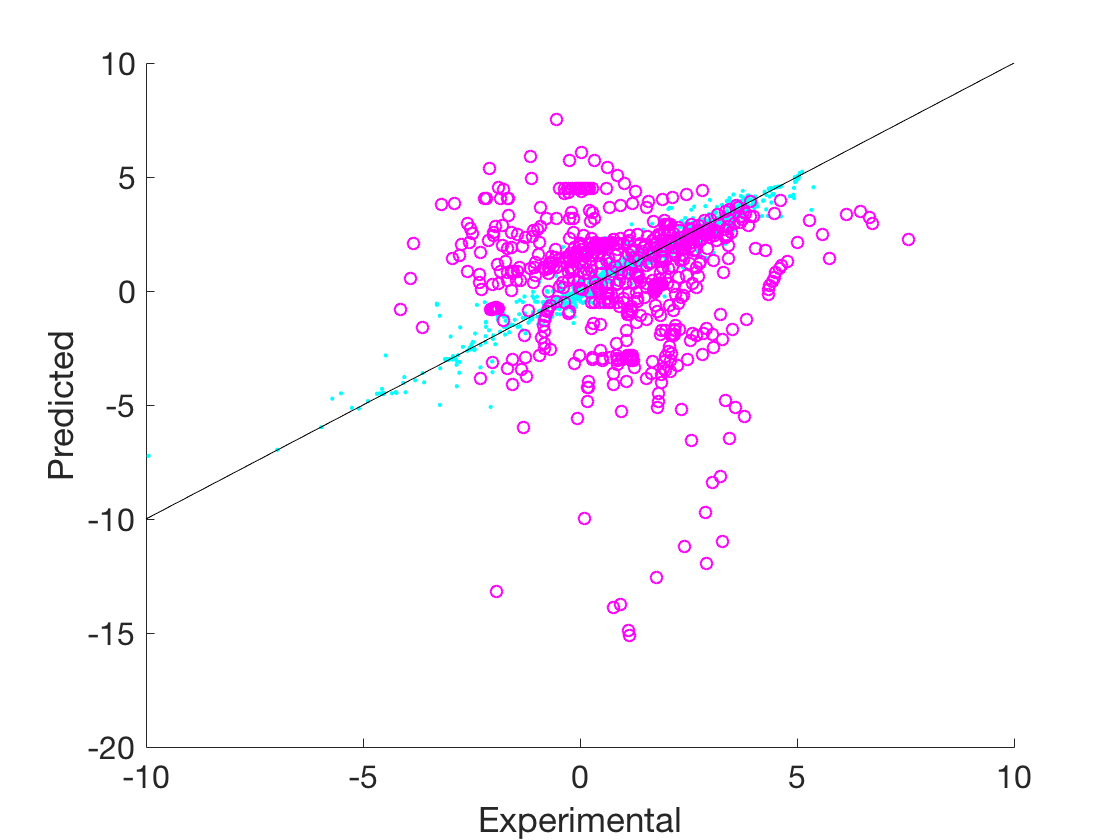
\includegraphics[width=0.5\textwidth]{Results/MainANN/WithAuPtCeO2_Superimposed.png}
	        \caption{ANN performance with \ce{Au/CeO2} and \ce{Pt/CeO2} instances}
	        \label{fig:Main NN with Au,Pt/CeO2}
	        \floatfoot{ {\color{cyan} $\bullet$} - Training Data, {\color{magenta} $\circ$} - \ce{Au/CeO2} and \ce{Pt/CeO2} Data }
		\end{figure}
	\FloatBarrier

%% -----------------------------------------------------------------------------
%% -----------------------------------------------------------------------------
\section{Analysis of Fitting Untrained Data}
Using continuous attributes to relate naturally categorical data should theoretically allow for predictions on materials that were not present in the original training data set. To test this, networks were trained with the original training data set (excluding \ce{Au/CeO2} and \ce{Pt/CeO2}), neglecting any instances with a given catalyst property (i.e., leaving out all attributes with Cu as the primary metal). The ability of the ANN to interpolate within the domain for unique catalysts was then evaluated by using the excluded data to compare the experimental forward rate to the predicted forward rate.

For all catalyst components explored below, it appears that an increase in the number of data points withheld increases prediction error. For cases such as \ce{Al2O3}, where nearly 30\% of the training data set is withheld, it may be expected that the resulting ANN is not nearly as robust.

	\subsection{Primary Metals}
	This was performed for all of the primary metals except Pt, due to the large number of instances with Pt-catalysts (1193 instances), given in figure \ref{fig:primary metal exclusion}. Acceptable predictions were observed for the primary metals Ir, Cu, Rh and Ru. However, the model did not successfully interpolate within the domain for Au and Pd. This could be attributed to either the number of data points, 99 for Au and 105 for Pd. 

	It is suggested that the lack of fit for Au is due to an alteration to the domain, resulting from the segregation of the \ce{Au} instances. Au has the weakest of the binding energy (-3.06eV) of all the primary metals considered. By removing \ce{Au} from the training data set, we reduce the domain from  $-6.46 < BE_C < -3.06 eV$ to $-6.46 < BE_C < -3.75 eV$. Thus, the model's predictions are extrapolations outside of the training domain, which is well understood to lead to a decrease is predictive accuracy \cite{Corma_2003_2}. 

	For Pd it appears the prediction segregates into two dominant groups, one which follows the scaling relation and another that deviates. The predicted rate for the deviating data was much larger than the expected rate. Unlike the \ce{Au} justification, the binding energy attribute for Pd is in the middle of the data set (-5.62eV). Multiple factors may contribute to this result. It is possible that the data cluster not following the scaling relationship has an unusual feature that was not within the domain space upon removal of all instances with \ce{Pd} as the primary metal. It is also possible that the catalyst behaves more like the \ce{Au/CeO2} and \ce{Pt/CeO2} catalysts described above, due to some methodological difference in the catalyst preparation. Regardless, additional work would be needed to confirm the source of this discrepancy. 

	\begin{figure}[!htbp]
	    \centering
	    \begin{subfigure}[b]{0.35\textwidth}
	        \centering
	        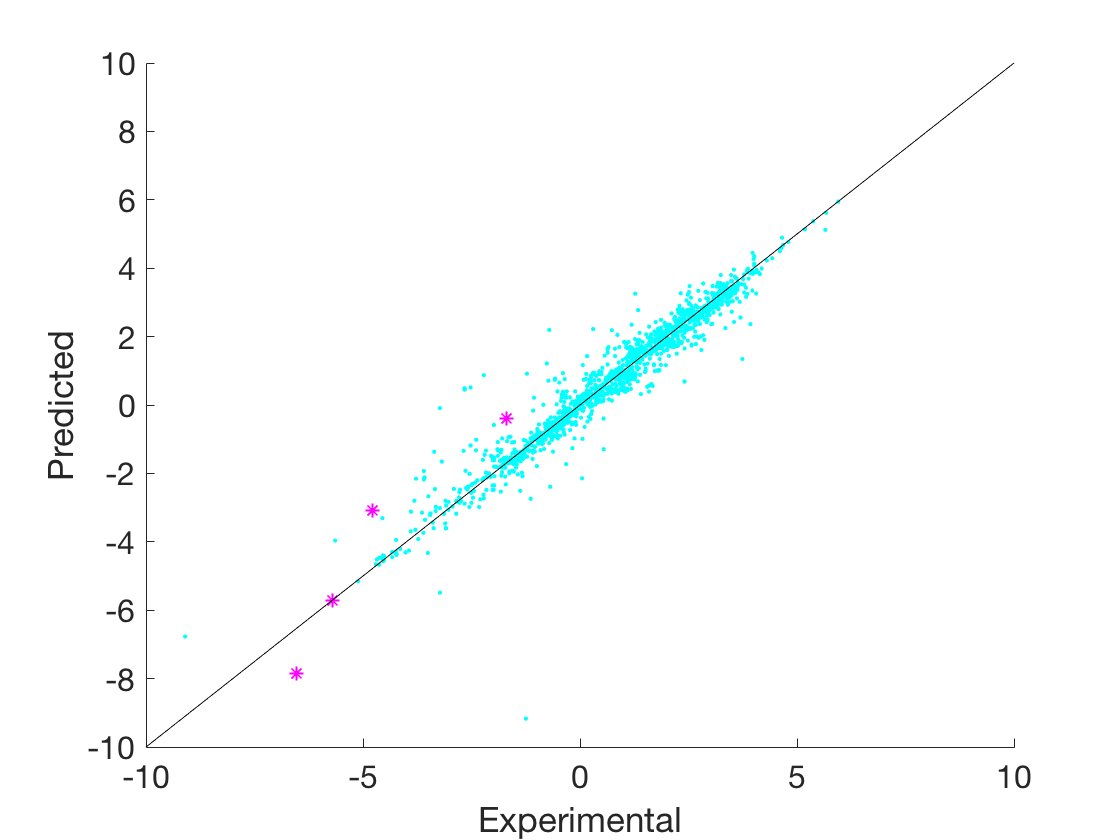
\includegraphics[width=\textwidth]{Results/PrimaryMetal/Ir_PredictionResults.png}
	        \caption{Ir}
	        \label{fig:non-norm_dist, Ir}
	    \end{subfigure}
	    \begin{subfigure}[b]{0.35\textwidth}
	        \centering
	        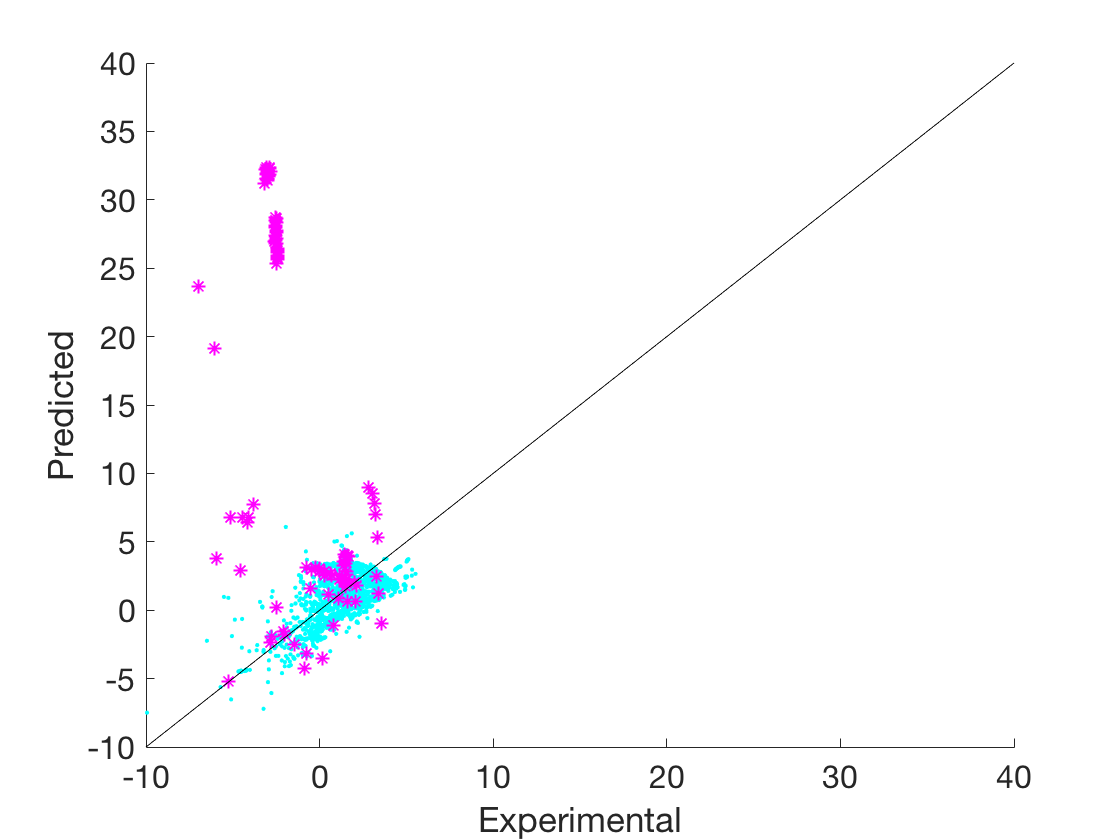
\includegraphics[width=\textwidth]{Results/PrimaryMetal/Pd_PredictionResults.png}
	        \caption{Pd}
	        \label{fig:norm_dist, Pd}
	    \end{subfigure}
	    \begin{subfigure}[b]{0.35\textwidth}
	        \centering
	        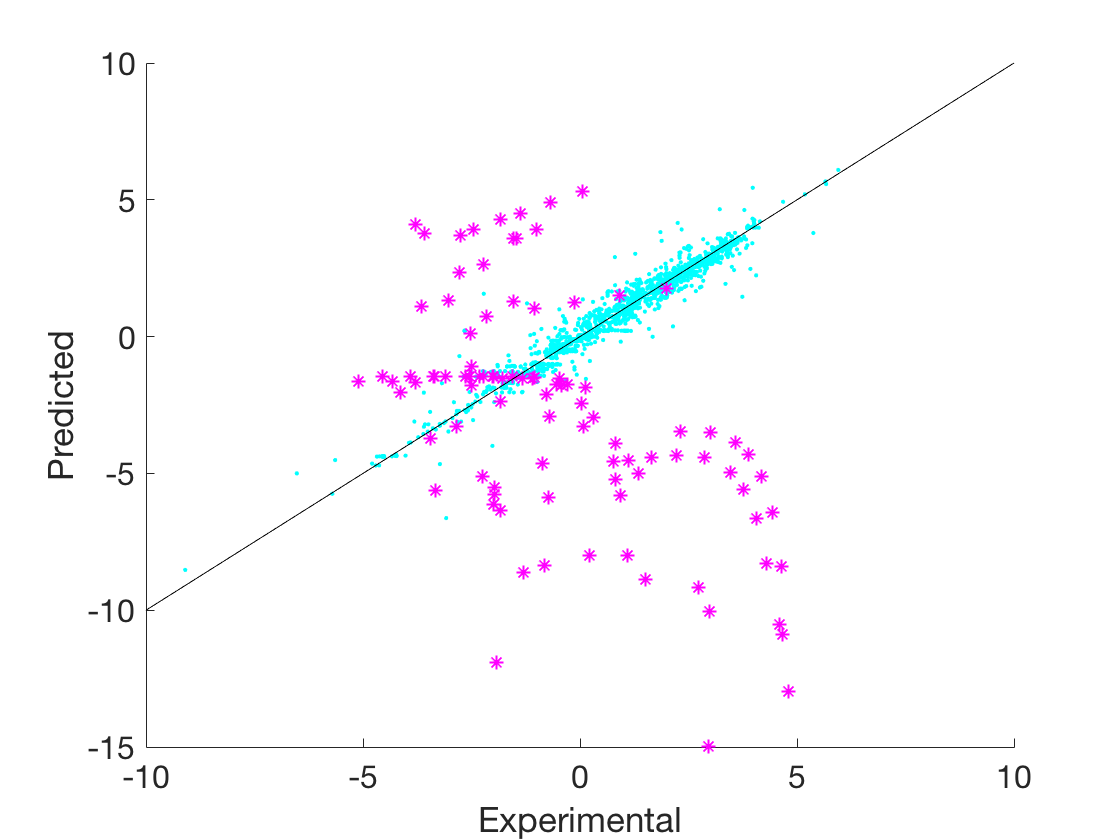
\includegraphics[width=\textwidth]{Results/PrimaryMetal/Au_PredictionResults.png}
	        \caption{Au}
	        \label{fig:norm_dist, Au}
	    \end{subfigure}
	    \begin{subfigure}[b]{0.35\textwidth}
	        \centering
	        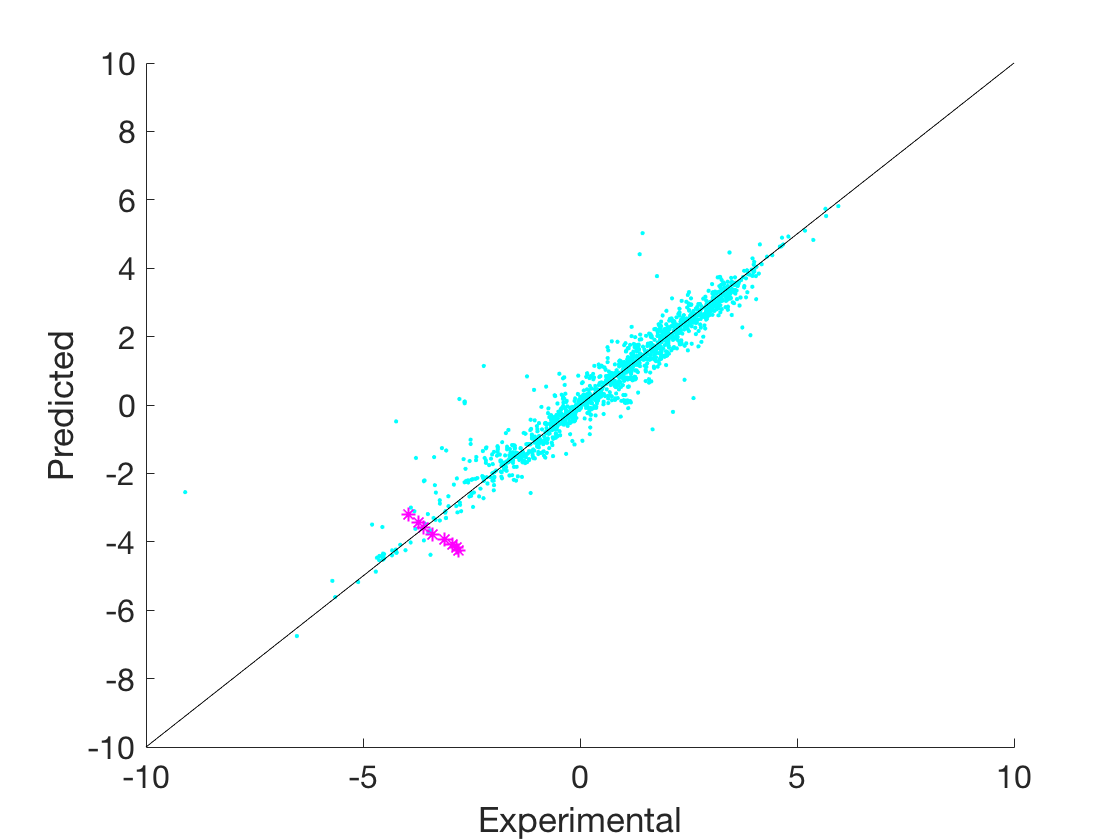
\includegraphics[width=\textwidth]{Results/PrimaryMetal/Cu_PredictionResults.png}
	        \caption{Cu}
	        \label{fig:norm_dist, Cu}
	    \end{subfigure}
	    \begin{subfigure}[b]{0.35\textwidth}
	        \centering
	        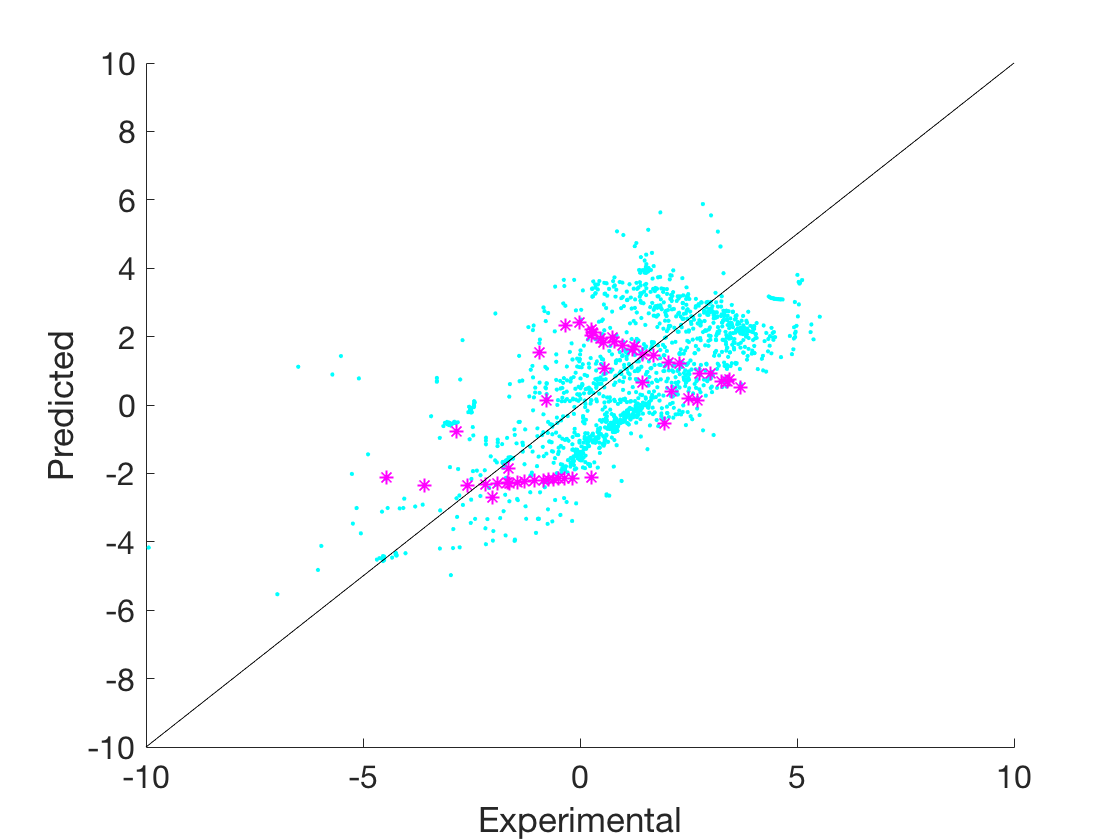
\includegraphics[width=\textwidth]{Results/PrimaryMetal/Rh_PredictionResults.png}
	        \caption{Rh}
	        \label{fig:norm_dist, Rh}
	    \end{subfigure}
	    \begin{subfigure}[b]{0.35\textwidth}
	        \centering
	        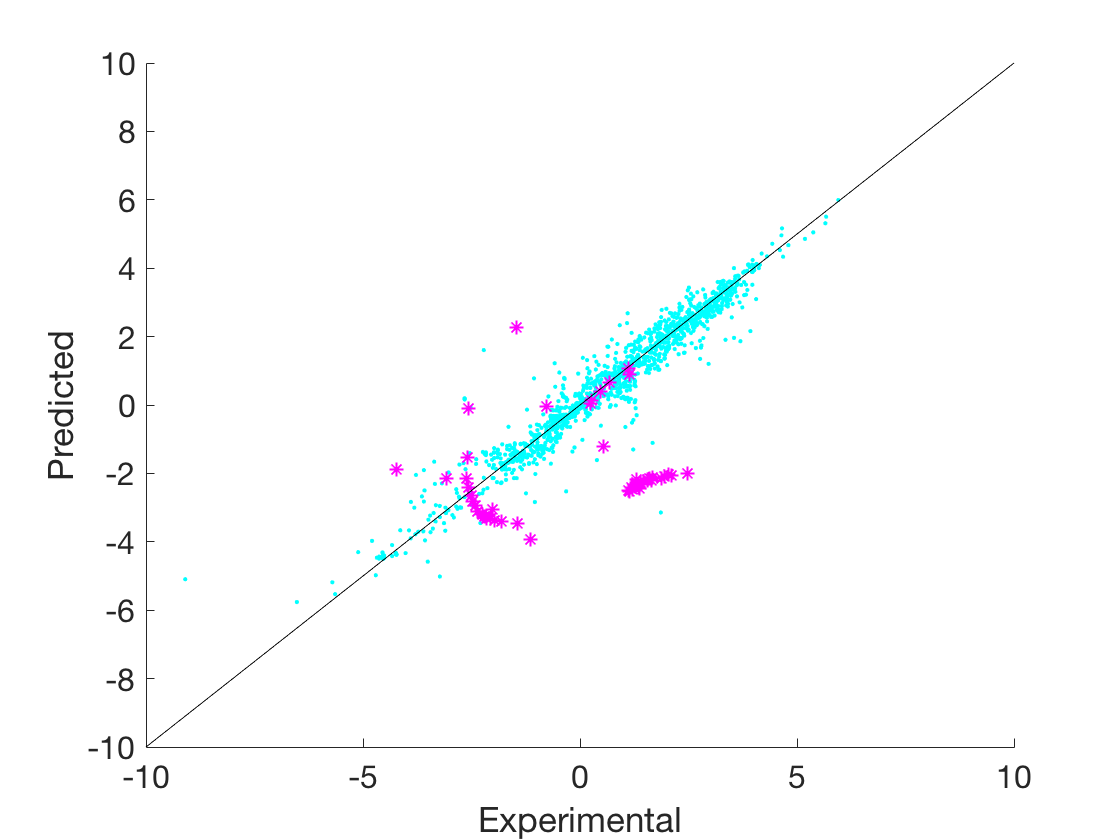
\includegraphics[width=\textwidth]{Results/PrimaryMetal/Ru_PredictionResults.png}
	        \caption{Ru}
	        \label{fig:norm_dist, Ru}
	    \end{subfigure}
	    \caption{Primary Metal Interpolation Results}
	    \label{fig:primary metal exclusion}
	    \floatfoot{ {\color{cyan} $\bullet$} - Training Data, {\color{magenta} $\bullet$} - Testing with Indicated Primary Metal Data }
	\end{figure}
	\FloatBarrier


	\subsection{Supports}
	The procedure was repeated for instances of varying supports (\ce{Al2O3}, \ce{CaO}, \ce{Co3O4}, \ce{HfO2}, \ce{La2O3}, \ce{SiO2}, \ce{Y2O3}), selectively choosing supports that span the domain. \ref{fig:support exclusion}. Of the supports explored, only \ce{Al2O3} and \ce{SiO2} yielded poor predictions. It is suggested that in the case of \ce{Al2O3} supports removing the 556 data points negatively impacted ANN training, as previously discussed. For \ce{SiO2} 29 data points were removed. Thus, it is unlikely that the quantity of data removed impacted the training. However, \ce{SiO2} had the maximum support electronegativity (1.9, Pauling Scale) in the domain. Similar to the argument for \ce{Au}, it is likely that removal of these data points decreased the domain space and the model had to extrapolate to make predictions. As a result, the error of the predictions increased. 
	\begin{figure}[!htbp]
	    \centering
	    \begin{subfigure}[b]{0.3\textwidth}
	        \centering
	        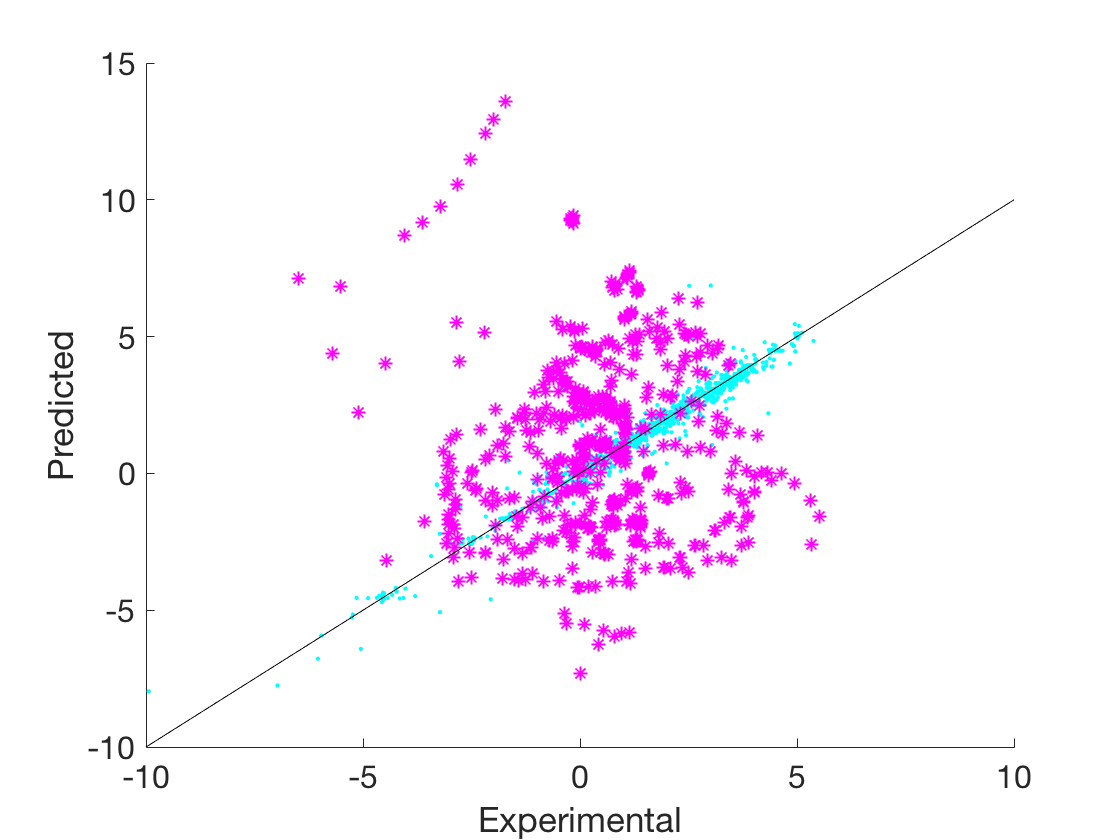
\includegraphics[width=\textwidth]{Results/Supports/Al2O3_PredictionResults.png}
	        \caption{\ce{Al2O3}}
	        \label{fig:non-norm_dist, Al2O3}
	    \end{subfigure}
	    \begin{subfigure}[b]{0.3\textwidth}
	        \centering
	        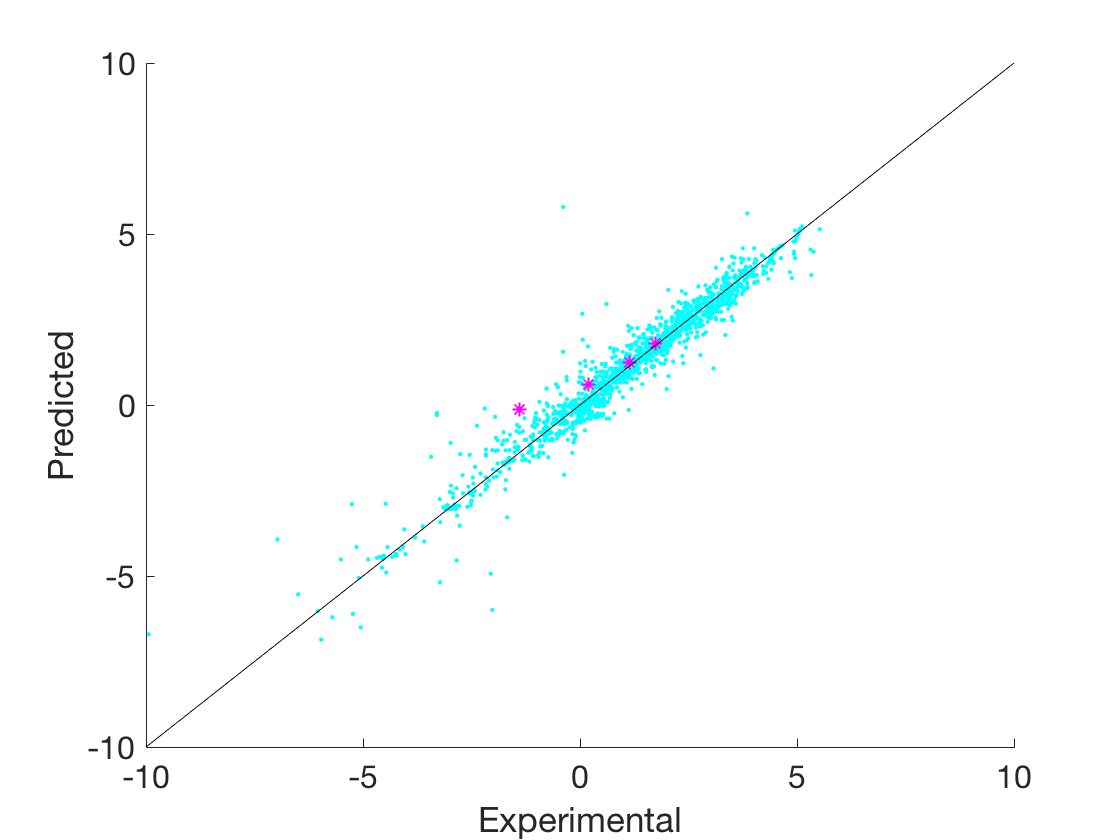
\includegraphics[width=\textwidth]{Results/Supports/CaO_PredictionResults.png}
	        \caption{\ce{CaO}}
	        \label{fig:norm_dist, CaO}
	    \end{subfigure}
	    \begin{subfigure}[b]{0.3\textwidth}
	        \centering
	        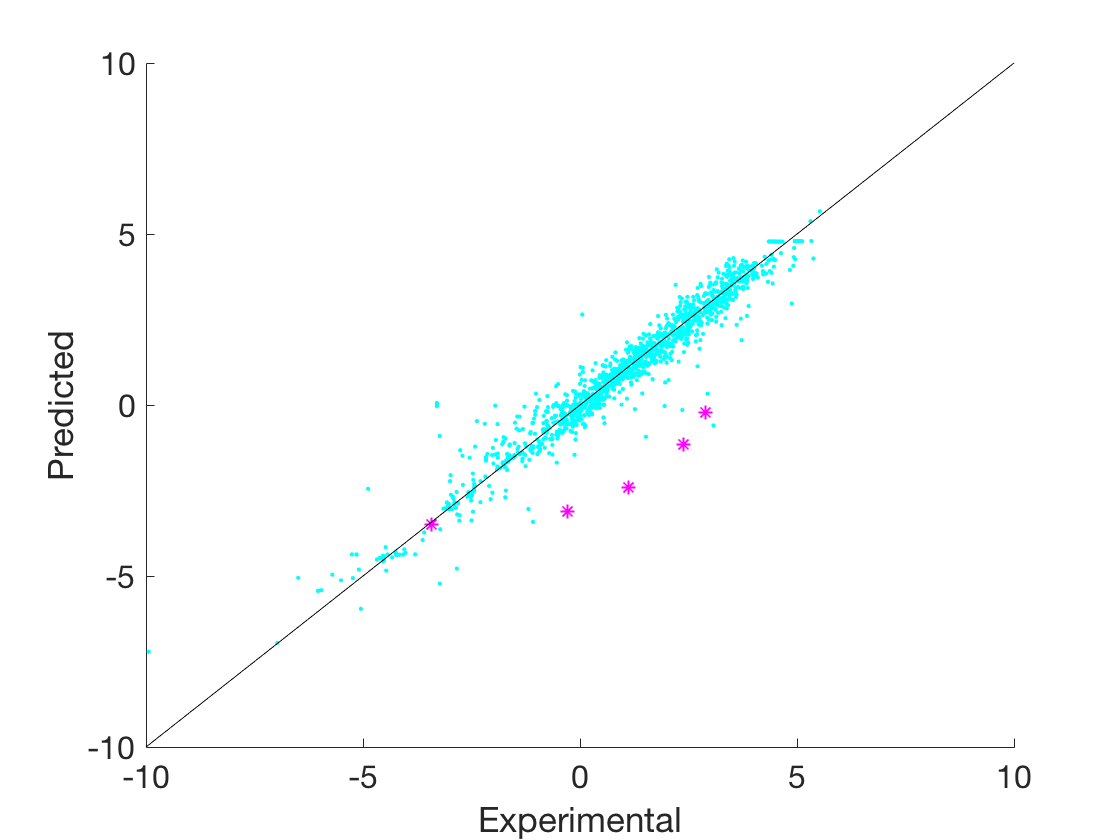
\includegraphics[width=\textwidth]{Results/Supports/Co3O4_PredictionResults.png}
	        \caption{\ce{Co3O4}}
	        \label{fig:norm_dist, Co3O4}
	    \end{subfigure}
	    \begin{subfigure}[b]{0.3\textwidth}
	        \centering
	        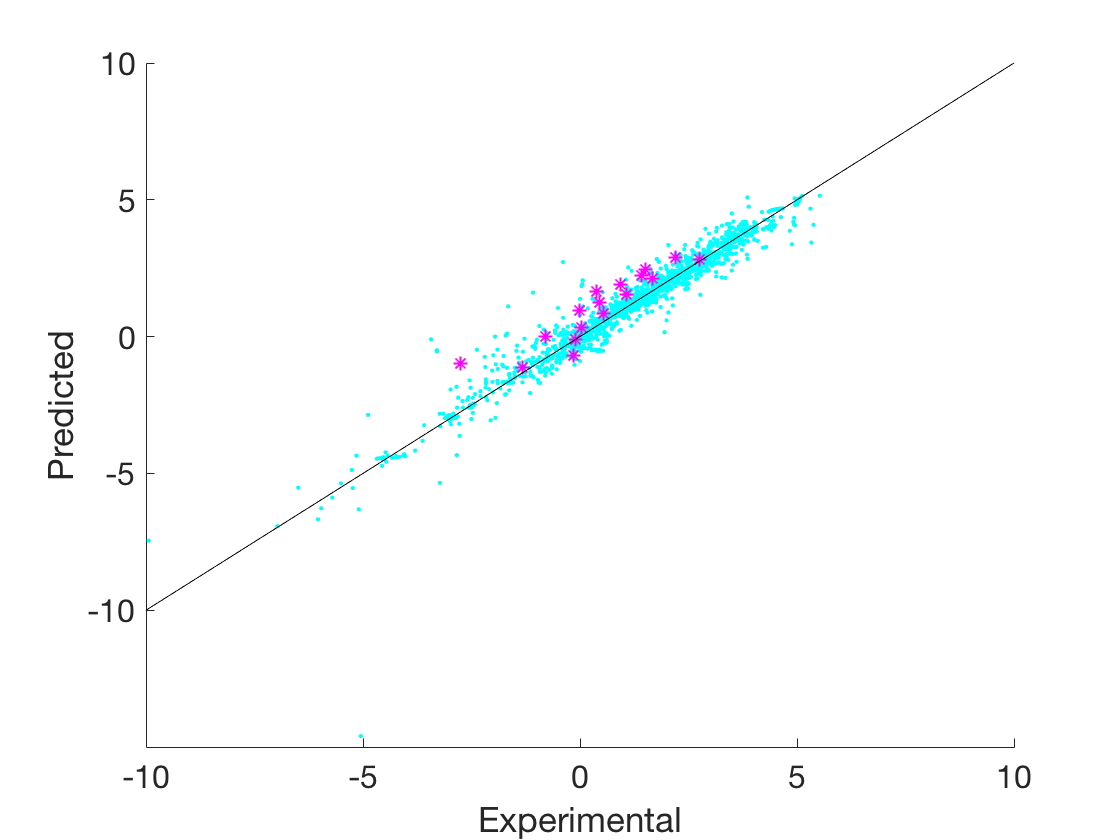
\includegraphics[width=\textwidth]{Results/Supports/HfO2_PredictionResults.png}
	        \caption{\ce{HfO2}}
	        \label{fig:norm_dist, HfO2}
	    \end{subfigure}
	    \begin{subfigure}[b]{0.3\textwidth}
	        \centering
	        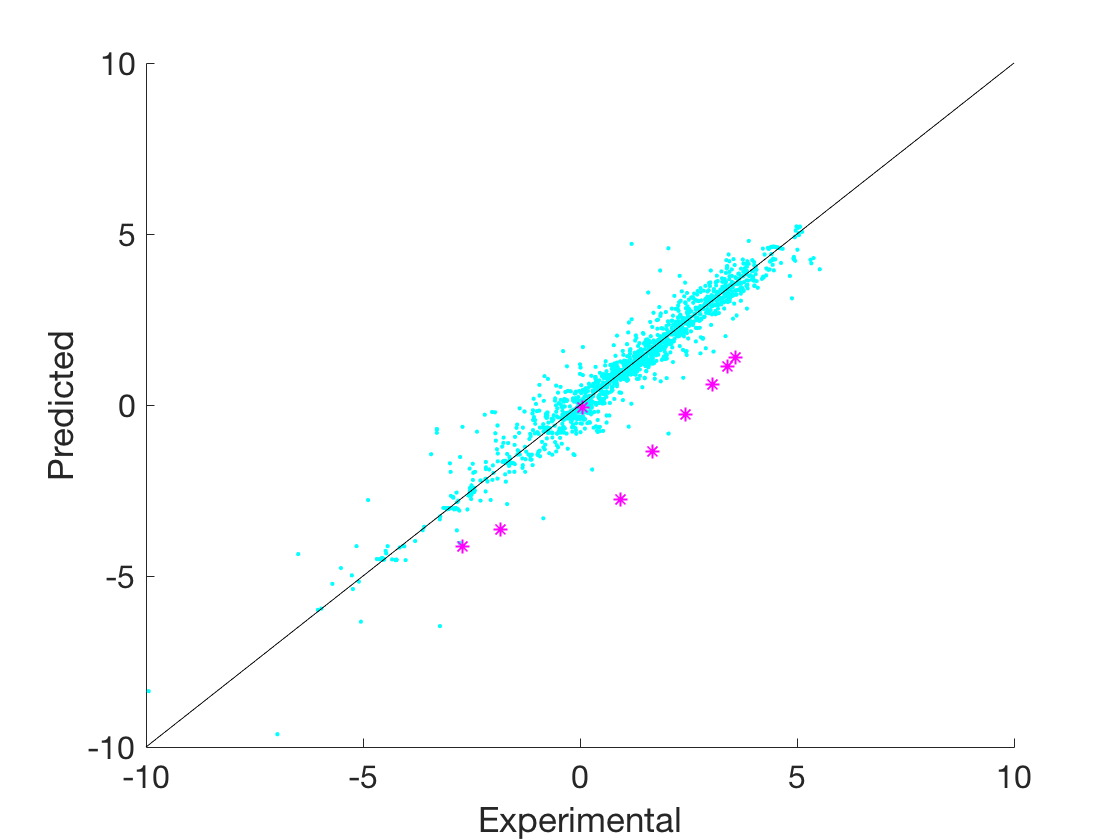
\includegraphics[width=\textwidth]{Results/Supports/La2O3_PredictionResults.png}
	        \caption{\ce{La2O3}}
	        \label{fig:norm_dist, La2O3}
	    \end{subfigure}
	    \begin{subfigure}[b]{0.3\textwidth}
	        \centering
	        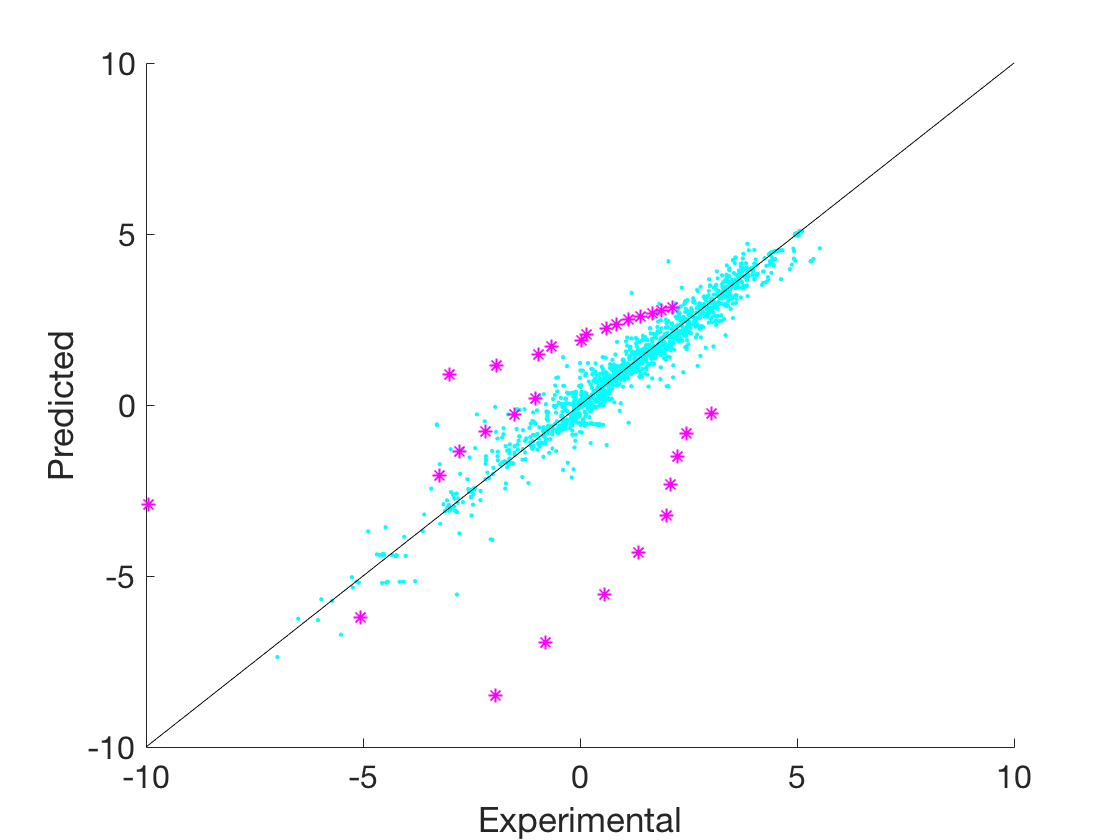
\includegraphics[width=\textwidth]{Results/Supports/SiO2_PredictionResults.png}
	        \caption{\ce{SiO2}}
	        \label{fig:norm_dist, SiO2}
	    \end{subfigure}
	    \begin{subfigure}[b]{0.3\textwidth}
	        \centering
	        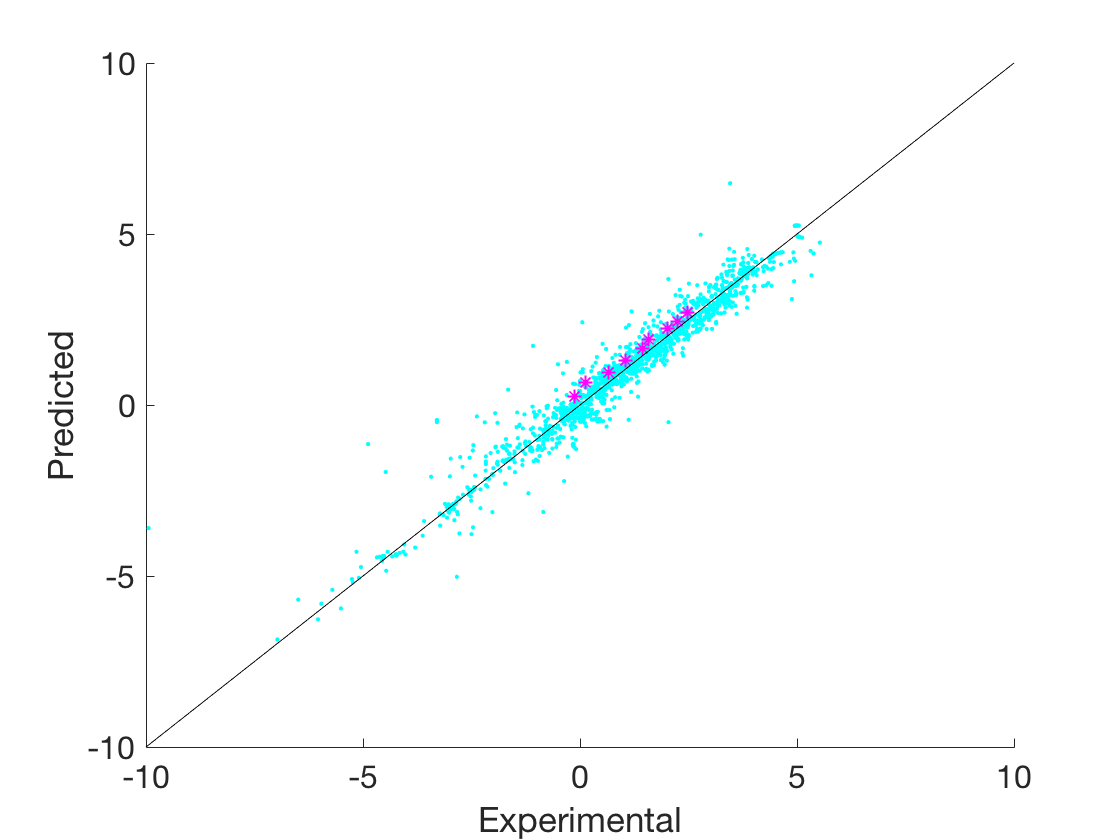
\includegraphics[width=\textwidth]{Results/Supports/Y2O3_PredictionResults.png}
	        \caption{\ce{Y2O3}}
	        \label{fig:norm_dist, Y2O3}
	    \end{subfigure}
	    \caption{Support Interpolation Results}
	    \label{fig:support exclusion}
	    \floatfoot{ {\color{cyan} $\bullet$} - Training Data, {\color{magenta} $\bullet$} - Testing with Indicated Support Data }
	\end{figure}
	\FloatBarrier


	\subsection{Promoters}
	The ability to predict promoter contributions was also evaluated by considering the promoters \ce{Ca}, \ce{Ce}, \ce{Cs}, \ce{Fe}, \ce{Gd}, \ce{La}, \ce{Re}, shown in figure \ref{fig:promoter exclusion}. Again, the group with the largest number of instances, Ce (297 instances) demonstrated the largest prediction error, although the associated attributes (electronegativity = 1.12, Charge/ionic Radius = 0.46) were well within the domain. Therefore, it is suggested that either the number of data points removed affected training performance or using a \ce{Ce} promoter alters the reaction mechanism, resulting in a catalyst that breaks the scaling relation. 

	\begin{figure}[!htbp]
	    \centering
	    \begin{subfigure}[b]{0.32\textwidth}
	        \centering
	        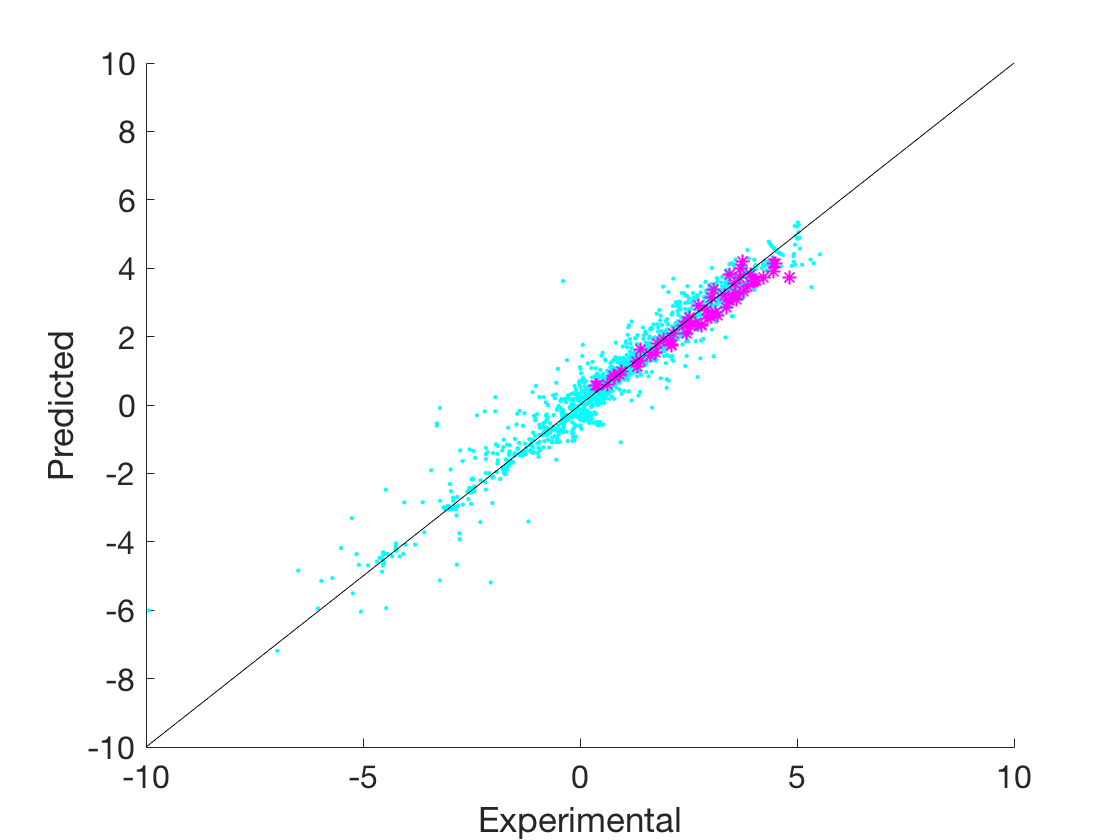
\includegraphics[width=\textwidth]{Results/Promoter/Ca_PredictionResults.png}
	        \caption{Ca}	    
	        \end{subfigure}
	    \begin{subfigure}[b]{0.32\textwidth}
	        \centering
	        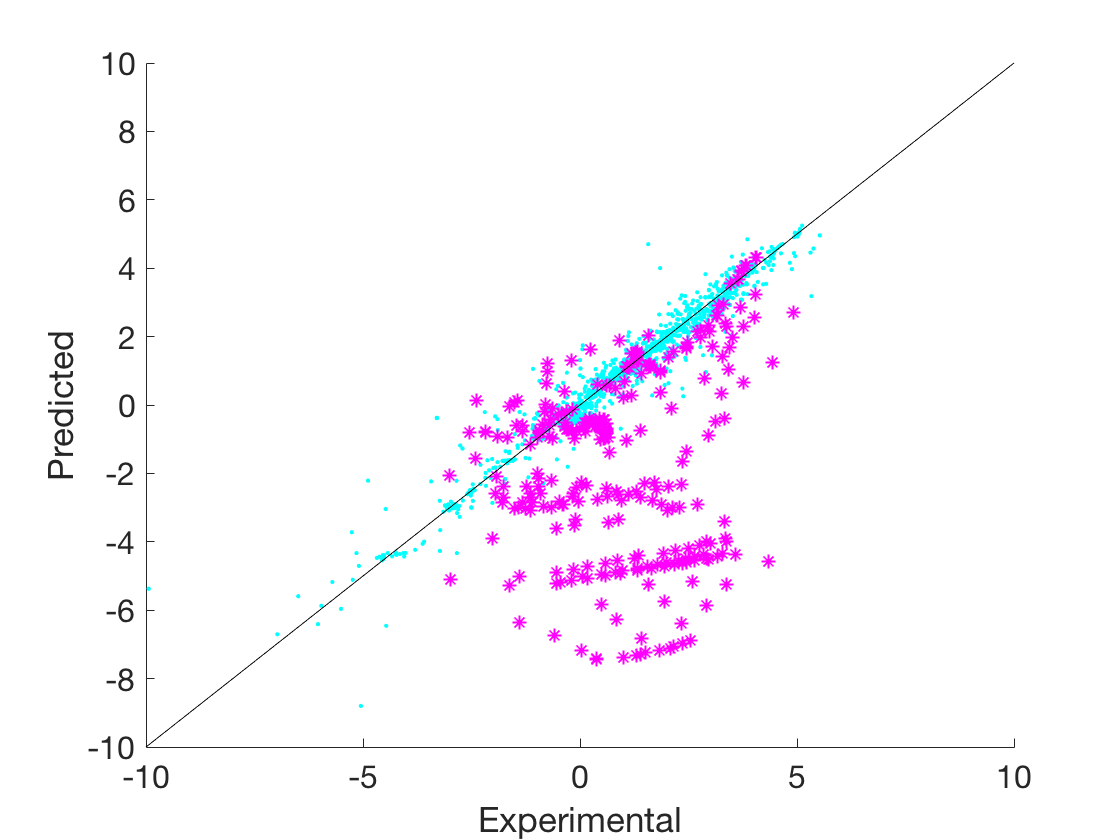
\includegraphics[width=\textwidth]{Results/Promoter/Ce_PredictionResults.png}
	        \caption{Ce}
	    \end{subfigure}
	    \begin{subfigure}[b]{0.32\textwidth}
	        \centering
	        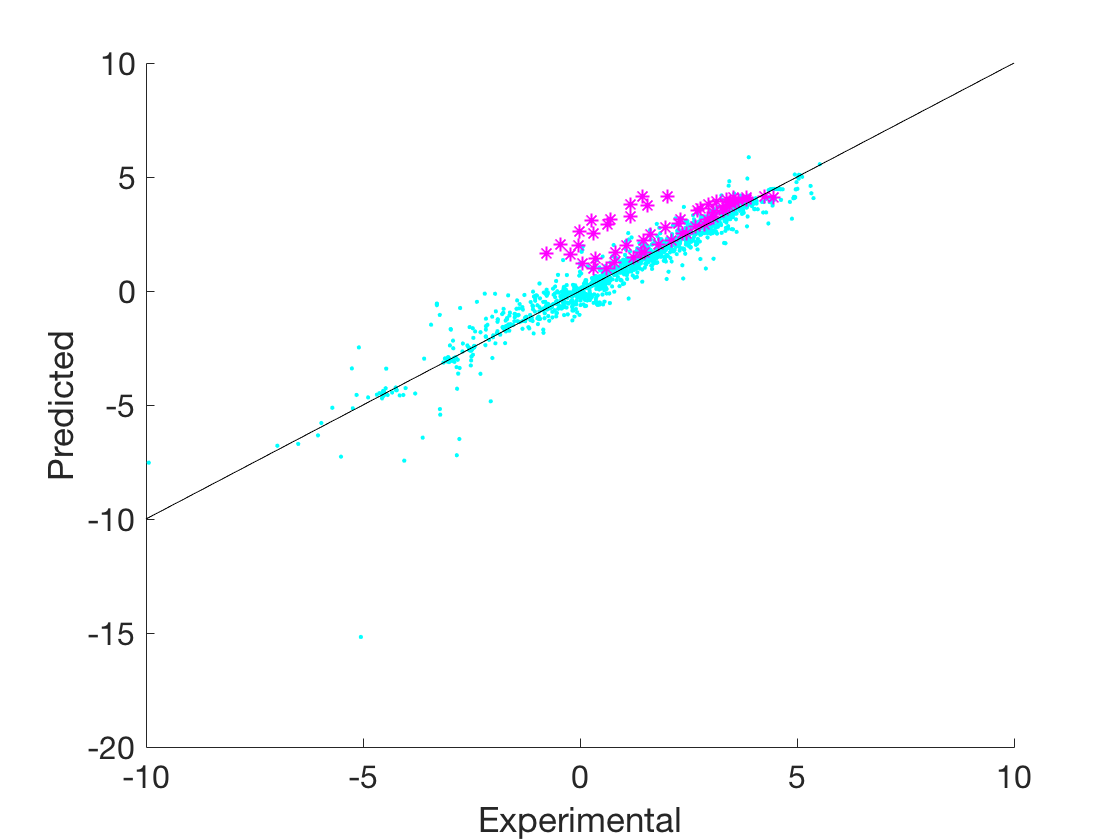
\includegraphics[width=\textwidth]{Results/Promoter/Cs_PredictionResults.png}
	        \caption{Cs}
	    \end{subfigure}
	    \begin{subfigure}[b]{0.32\textwidth}
	        \centering
	        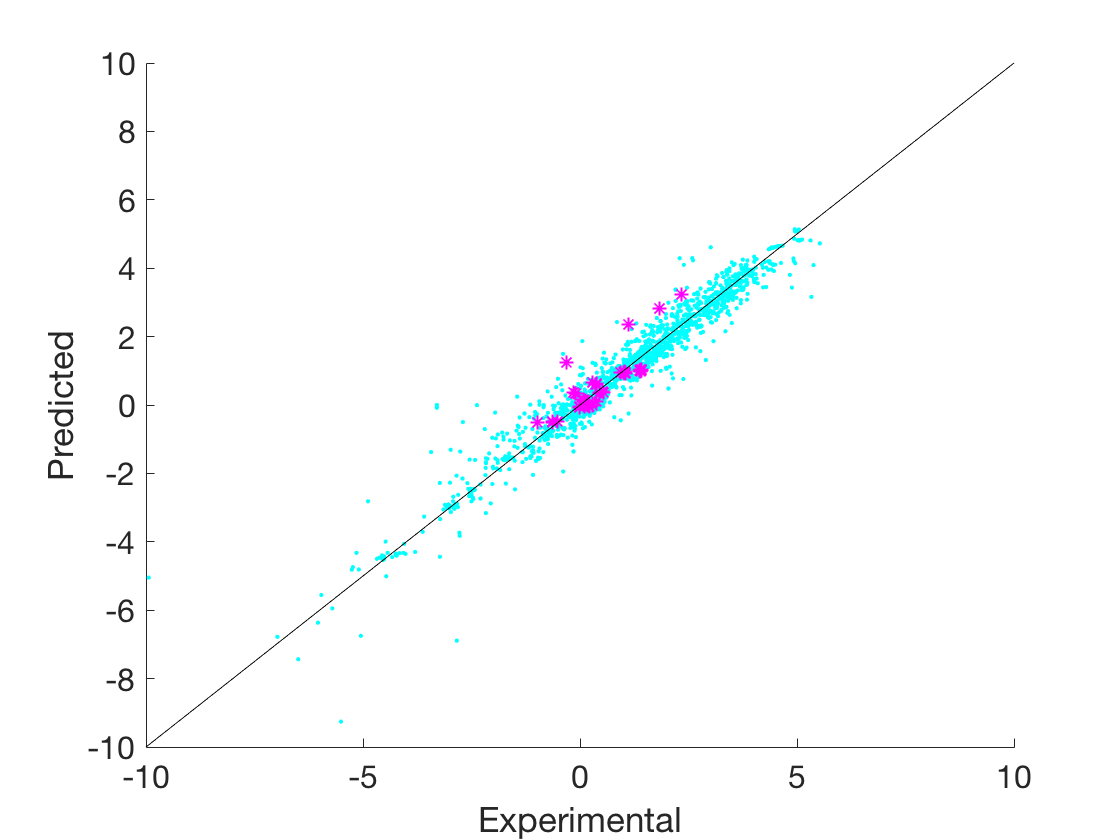
\includegraphics[width=\textwidth]{Results/Promoter/Fe_PredictionResults.png}
	        \caption{Fe}
	    \end{subfigure}
	    \begin{subfigure}[b]{0.32\textwidth}
	        \centering
	        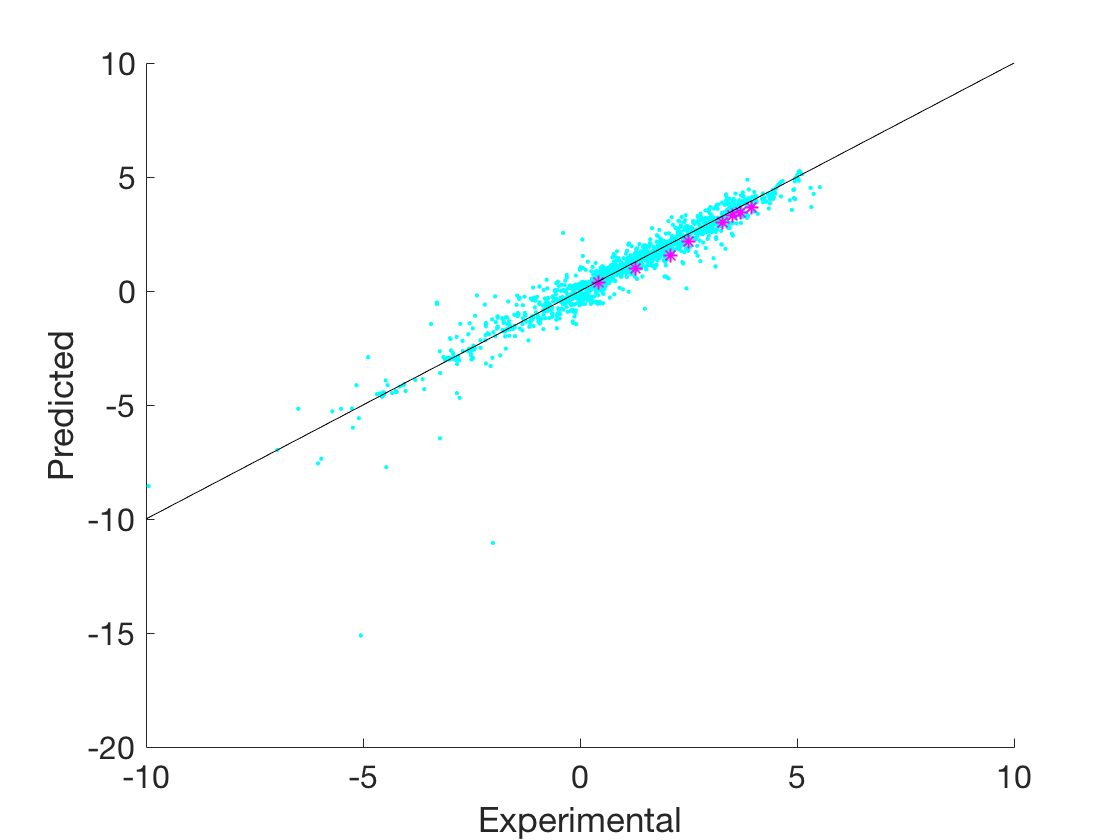
\includegraphics[width=\textwidth]{Results/Promoter/Gd_PredictionResults.png}
	        \caption{Gd}
	    \end{subfigure}
	    \begin{subfigure}[b]{0.32\textwidth}
	        \centering
	        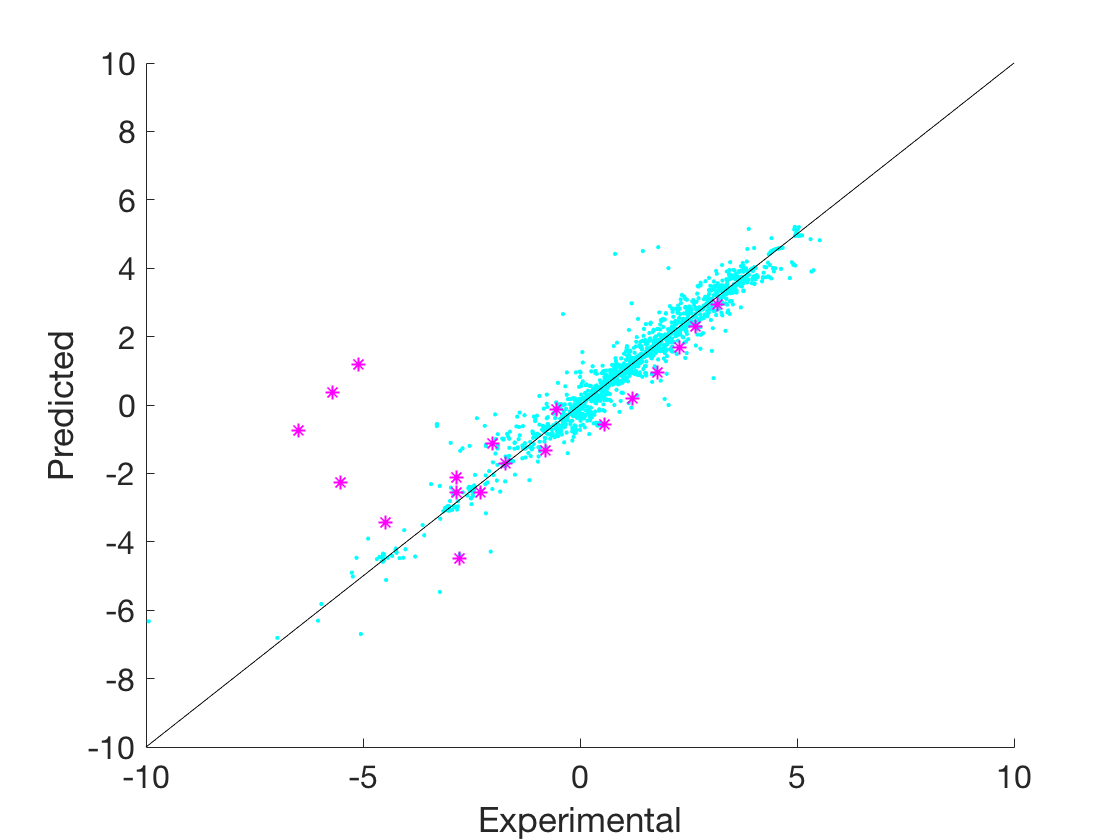
\includegraphics[width=\textwidth]{Results/Promoter/La_PredictionResults.png}
	        \caption{La}
	    \end{subfigure}
	    \begin{subfigure}[b]{0.32\textwidth}
	        \centering
	        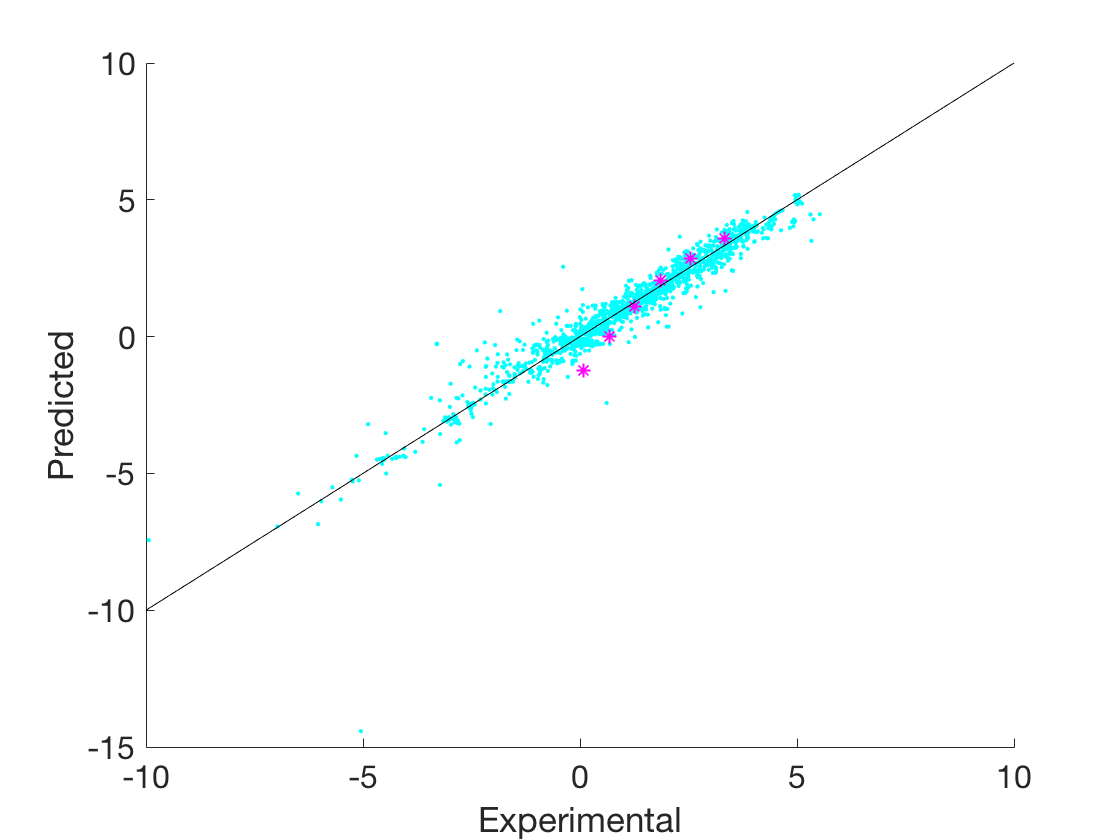
\includegraphics[width=\textwidth]{Results/Promoter/Re_PredictionResults.png}
	        \caption{Re}
	    \end{subfigure}
	    \caption{Promoter Interpolation Results}
	    \label{fig:promoter exclusion}
	    \floatfoot{ {\color{cyan} $\bullet$} - Training Data, {\color{magenta} $\bullet$} - Testing with Indicated Promoter Data }
	\end{figure}
	\FloatBarrier

